\documentclass[a4paper, 12pt]{article}
\usepackage[utf8]{inputenc}
\renewcommand\familydefault{\sfdefault}
\usepackage[T1]{fontenc}
\usepackage[francais]{babel}
\usepackage[left=2.5cm,top=2.5cm,right=2.5cm,bottom=2.5cm]{geometry}
\usepackage{graphicx}
\usepackage{minted}
\usemintedstyle{colorful}
\usepackage{float}
\floatplacement{figure}{H}
\usepackage{authblk}
\usepackage{enumitem}
\usepackage{hyperref} 
\hypersetup{
	colorlinks,
	citecolor=black,
	filecolor=black,
	linkcolor=black,
	urlcolor=blue
}

\usepackage{caption}
\newenvironment{code}{\captionsetup{type=listing}}{}
\usepackage{array}
\usepackage{etoolbox} 
\patchcmd{\thebibliography}{\section*{\refname}}{}{}{}

\begin{document}

\title{BibApp Hepia} 
\author{Steven Liatti} 
\affil{\small Projet de semestre - Prof. Mickaël Hoerdt} 
\affil{\small Hepia ITI 3\up{ème} année} 
\maketitle
\newpage

\tableofcontents
\listoffigures
% \renewcommand\listoflistingscaption{Table des scripts de code}
% \listoflistings
\newpage

% \mintinline{java}{GameView}

\section{Introduction}
\subsection{Besoins de la bibliothèque}
La bibliothèque de l'hepia aimerait attirer plus de monde en créant du contenu personnalisé autour de son 
catalogue d'ouvrages et revues par le biais d'un site/application mobile. Voici les besoins listés plus 
précisement :
\begin{itemize}
	\item Résumé d'un nouveau livre arrivé à la bibliothèque (nouveautés)
	\item Coups de coeur des bibliothécaires sur les ouvrages présents
	\item Revues de presse des périodiques
	\item Ajouter les images des couvertures scannées par la bibliothèque
\end{itemize}
Toutes ces actions doivent pouvoir être réalisées via le site web en mode administrateur. Les opérations de 
création, récupération, modification et suppression de contenu (CRUD) sont nécessaires. Un mode utilisateur, ou visiteur, 
permet de consulter le contenu, depuis un ordinateur ou un appareil mobile. L'idée est de créer une source 
de contenus basée sur le catalogue Nebis et augmentée par les ajouts des bibliothécaires.

\section{Technologies utilisées}
\subsection{Ionic}
\subsection{Node.js}
\subsection{MongoDB}
\subsection{JSON Web Tokens}

\section{Tutoriel sur Ionic}
\textit{Voir BibApp - Ionic.md (pour l'instant)}

% p{.5\linewidth}

% \begin{table}[h]
% 	\begin{tabular}{|c|c|c|c|}	\hline
% 		\textbf{Besoin}	& \textbf{Actions} & \textbf{Priorité} & \textbf{Temps demandé} \\ \hline
% 		&&& \\ \hline
% 		\end{tabular}
% \end{table}

\section{Architecture}
Actuellement, le catalogue Nebis est utilisé par la bibliothèque. Cependant, il sera abandonné dans quelques 
années pour un nouveau catalogue, encore inconnu à ce jour. L'objectif étant de réaliser une web app pérenne, 
il faut pouvoir s'adapter à ce changement. Voici ci-dessous l'architecture globale de l'application :
\begin{figure}
	\begin{center}
		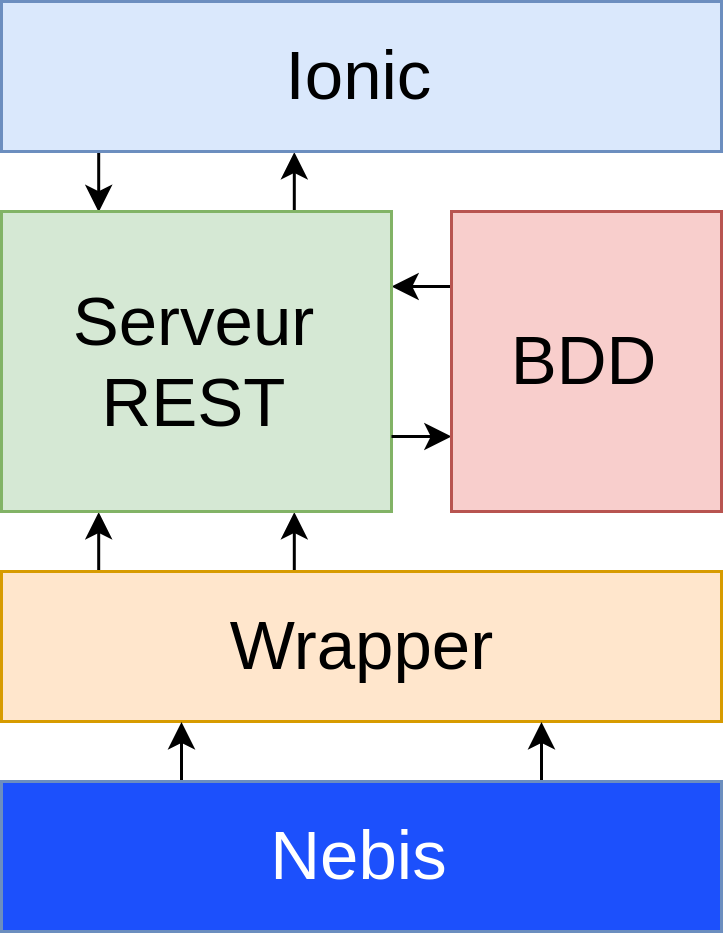
\includegraphics[width=0.5\textwidth]{images/architecture.png}
	\end{center}
	\caption{Architecture globale de la web app}
\end{figure}
Le Wrapper et le serveur REST seront faits en Node.js. La base de données sera faite avec MongoDB.

\subsection{Wrapper}
Ce module fait le pont entre les données issues d'un catalogue et le serveur REST. Son utilité principale est 
de s'adapter au catalogue utilisé : si le catalogue est amené à changer ou à disparaître au profit d'un autre, 
il suffira de modifier ce Wrapper pour continuer à faire fonctionner l'application. Il devra au minimum fournir :
\begin{itemize}
	\item La liste des nouveautés
	\item Les informations de base sur les ouvrages
	\item La recherche d'une oeuvre par ISBN et/ou d'autres critères
\end{itemize}


\subsection{Serveur REST}
Ce serveur offre les services suivants :
\begin{itemize}
	\item CRUD pour les infos de base des oeuvres (Nebis)
	\item CRUD pour les résumés/commentaires des livres
	\item CRUD pour les coups de coeur des bibliothécaires
	\item CRUD pour les revues de presse
	\item CRUD pour les images scannées par les bibliothécaires
	\item Authentification et autorisations des utilisateurs
\end{itemize}

\subsection{Base de données}
La base de données sera liée au serveur REST, elle enregistrera le contenu produit par la bibliothèque.
\begin{figure}
	\begin{center}
		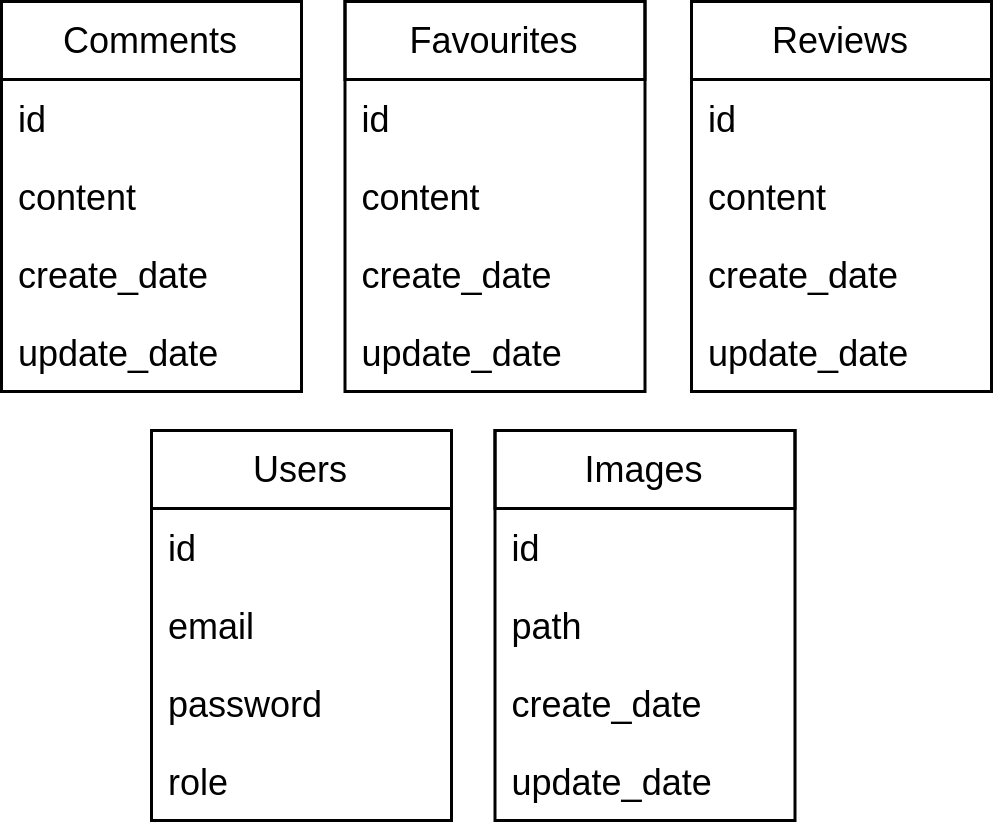
\includegraphics[width=0.9\textwidth]{images/bdd.png}
	\end{center}
	\caption{Schéma de la base de données}
\end{figure}
\textit{(Ce schéma est amené à évoluer)}

\subsection{Ionic}
Partie front-end de l'application, elle offrira côté utilisateur :
\begin{itemize}
	\item Page d'accueil, avec les sections "Nouveautés", "Coups de coeur" et "Revues de presse"
	\item Pour chaque section, une page listant les ouvrages ou périodiques avec infos de base 
		(Titre, auteur, etc. et image si fournie)
	\item Pour chaque entrée, la possibilité de cliquer dessus et consulter les infos Nebis et le contenu enrichi
\end{itemize}
Côté administrateur (ou rédacteur), les bibliothécaires pourront s'authentifier et auront une section supplémentaire, 
"Images", où ils pourront ajouter les scans des livres aux entrées existantes. Pour les autres sections, ils 
pourront ajouter le contenu correspondant aux entrées voulues. \cite{ref1}


\section{Réalisation}
\subsection{Captures d'écran}

\section{Conclusion}

\section{Annexes}

\section{Références}
\bibliographystyle{unsrt}
\bibliography{bib}

\end{document}
